\documentclass[hyperref={bookmarks=false},aspectratio=169]{beamer}
\usepackage{hyperref,ragged2e,amsmath,amssymb,url,bm}
\usepackage{graphicx,booktabs,array}
\usepackage{tikz}
\usetikzlibrary{arrows.meta,positioning,calc,shapes.geometric,decorations.pathreplacing,matrix}
\graphicspath{{crops/}}
\usetheme{Goettingen}
% --- Paleta: azul profundo, dorado y papiro crema ---
\definecolor{azul}{HTML}{15437C}
\definecolor{azuloscuro}{HTML}{0B1F3A}
\definecolor{celeste}{HTML}{5694D6}
\definecolor{dorado}{RGB}{196,154,60}
\definecolor{papiro}{RGB}{246,239,220}
\definecolor{gris}{RGB}{70,78,96}
\setbeamercolor{structure}{fg=azul}
\setbeamertemplate{sidebar canvas right}[vertical shading][top=azul,bottom=azuloscuro]
\setbeamercolor{title in sidebar}{fg=dorado}
\setbeamercolor{author in sidebar}{fg=papiro}
\setbeamercolor{section in sidebar}{fg=papiro}
\setbeamercolor{section in sidebar shaded}{fg=dorado!70!papiro}
\setbeamercolor{subsection in sidebar}{fg=papiro}
\setbeamercolor{subsection in sidebar shaded}{fg=dorado!70!papiro}
\let\raggedright\justifying
\setlength{\RaggedRightRightskip}{0pt plus 1fil}
\setbeamertemplate{background canvas}{
\includegraphics[width=\paperwidth,height=\paperheight]{papiro.jpg}}
\setbeamercolor{normal text}{fg=black!88!azuloscuro}
\setbeamercolor{frametitle}{fg=azul}
\setbeamerfont{frametitle}{series=\bfseries}
\setbeamertemplate{section in toc shaded}{\leavevmode{\color{gris}\inserttocsection}\par}
\setbeamercolor{title}{fg=azul}
\setbeamercolor{subtitle}{fg=gris}
\setbeamercolor{item projected}{bg=azul,fg=papiro}
\setbeamertemplate{itemize item}{\small\textcolor{dorado}{$\blacktriangleright$}}
\setbeamertemplate{navigation symbols}{}
% --- Español + hebreo + griego (XeLaTeX) ---
\usepackage[bidi=default]{babel}
\babelprovide[import,main]{spanish}
\babelprovide[import]{hebrew}
\babelprovide[import]{ancientgreek}
\babelfont[hebrew]{sf}[Path=fonts/, BoldFont=NotoHebrewSans-700.ttf]{NotoHebrewSans-400.ttf}
\babelfont[hebrew]{rm}[Path=fonts/, BoldFont=NotoHebrewSans-700.ttf]{NotoHebrewSans-400.ttf}
\babelfont[ancientgreek]{sf}[Path=fonts/]{GFSPorson.otf}
\babelfont[ancientgreek]{rm}[Path=fonts/]{GFSPorson.otf}
\newcommand{\heb}[1]{\mbox{\foreignlanguage{hebrew}{#1}}}
\newcommand{\grc}[1]{\foreignlanguage{ancientgreek}{#1}}
\newcommand{\SENOR}{S{\fontsize{0.78em}{1em}\selectfont EÑOR}}
% --- Citas (cuadro de un solo color), imágenes, referencias ---
\usepackage[most]{tcolorbox}
\newtcolorbox{cita}[1][]{enhanced, colback=azul!7!papiro, opacityback=0.85, colframe=azul,
  boxrule=0pt, leftrule=2.5pt, arc=0pt, left=6pt, right=6pt, top=4pt, bottom=4pt,
  before skip=4pt, after skip=6pt, fontupper=\small\itshape, #1}
\newcommand{\fuente}[1]{\par\hfill{\upshape\bfseries\footnotesize\textcolor{azul}{#1}}}
\makeatletter
\newcommand{\fotolado}[2]{%
  \begin{tikzpicture}[remember picture,overlay]
    \node[anchor=north east,inner sep=0pt] (foto) at ([xshift=-\beamer@sidebarwidth]current page.north east)
      {\includegraphics[height=\paperheight]{#1}};
    \node[anchor=south east,inner sep=2pt,text=papiro,fill=azuloscuro,fill opacity=0.6,text opacity=1,
      font=\fontsize{4.5}{5.5}\selectfont,align=right,text width=4.2cm] at ([xshift=-3pt,yshift=3pt]foto.south east)
      {\textit{Nota.} #2};
  \end{tikzpicture}}
\makeatother
\newcommand{\refapa}[1]{\par{\RaggedRight\hangindent=1.2em\hangafter=1\noindent #1\par}\vspace{3pt}}
\usepackage{xurl}\urlstyle{same}
\newcommand{\destacar}[1]{\textbf{\textcolor{azul}{#1}}}
\newcommand{\precision}[1]{{\footnotesize\color{gris}\textbf{Precisión:} #1}}
\tikzset{caja/.style={draw=azul,line width=0.8pt,fill=papiro,fill opacity=0.92,text opacity=1,rounded corners=3pt,inner sep=5pt,font=\scriptsize}}
\title[El Dios santo]{\bfseries{Santo, santo, santo}}
\subtitle{La santidad de Dios: la perfección que lo hace sin igual}
\author{}\institute{}\date{}
\titlegraphic{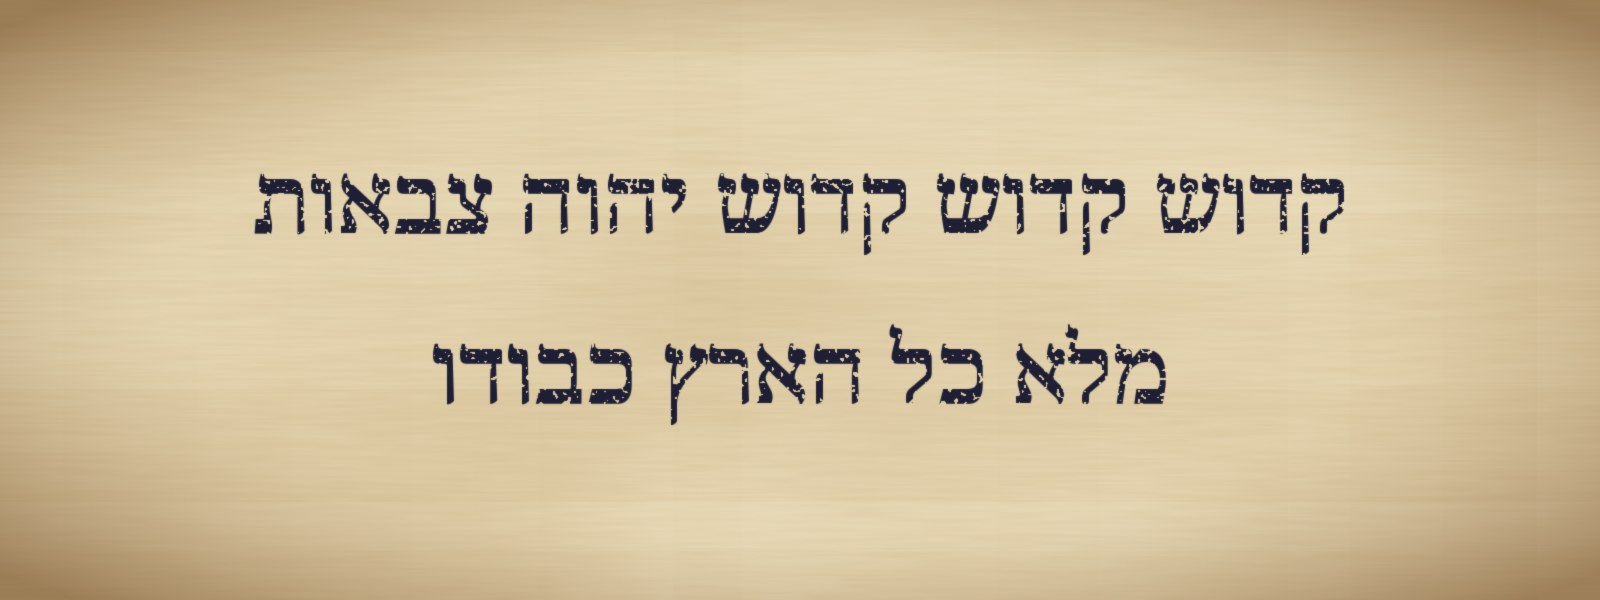
\includegraphics[width=0.80\linewidth,height=0.36\textheight,keepaspectratio]{portada.jpg}\\[-1pt]
  {\fontsize{5}{6}\selectfont\color{gris}\textit{Nota.} Elaboración propia: Is 6:3 en texto hebreo consonántico (BHS).}}
\begin{document}
\frame{\titlepage}

\begin{frame}\frametitle{Contenidos}\tableofcontents\end{frame}

% ------------------------------------------------------------------
\section{Isaías 6}

\begin{frame}{El año en que murió Uzías}
\begin{columns}[c,onlytextwidth]
\begin{column}{0.48\textwidth}
\small
\begin{itemize}
\item Hacia el 740~a.\,e.\,c. muere Uzías, rey de Judá durante 52 años (2~Cr 26:3).
\item Al final de su reinado entró al templo a quemar incienso, cosa reservada a los sacerdotes, y fue herido de lepra (2~Cr 26:16--21).
\item Ese mismo año Isaías ve otro trono: el del Rey que no muere.
\end{itemize}
\precision{el contraste entre el rey que profanó lo santo y el Rey santo es una lectura de varios intérpretes; Isaías no lo explicita.}
\end{column}
\begin{column}{0.50\textwidth}
\centering
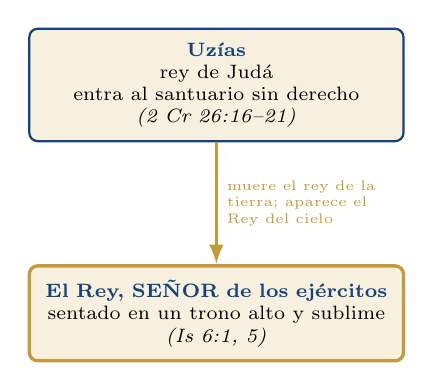
\begin{tikzpicture}[font=\scriptsize]
 \node[caja,text width=4.4cm,align=center] (u) at (0,1.6) {\textbf{\textcolor{azul}{Uzías}}\\ rey de Judá\\ entra al santuario sin derecho\\ \emph{(2 Cr 26:16--21)}};
 \node[caja,text width=4.4cm,align=center,draw=dorado,line width=1.2pt] (s) at (0,-1.3) {\textbf{\textcolor{azul}{El Rey, \SENOR{} de los ejércitos}}\\ sentado en un trono alto y sublime\\ \emph{(Is 6:1, 5)}};
 \draw[-{Latex[length=2.5mm]},line width=1pt,dorado] (u) -- node[right,text width=2.2cm,font=\tiny]{muere el rey de la tierra; aparece el Rey del cielo} (s);
\end{tikzpicture}
\end{column}
\end{columns}
\end{frame}

\begin{frame}{Texto ancla: Is 6:1--4}
\fotolado{panel_isaias6.jpg}{Elaboración propia: Is 6:3 y 1~S 2:2 en texto hebreo consonántico (BHS).}
\begin{columns}[c,onlytextwidth]
\begin{column}{0.58\textwidth}
\begin{cita}En el año que murió el rey Uzías vi yo al Señor sentado sobre un trono alto y sublime, y sus faldas llenaban el templo. Por encima de él había serafines; cada uno tenía seis alas; con dos cubrían sus rostros, con dos cubrían sus pies, y con dos volaban. Y el uno al otro daba voces, diciendo: Santo, santo, santo, \SENOR{} de los ejércitos; toda la tierra está llena de su gloria. Y los quiciales de las puertas se estremecieron con la voz del que clamaba, y la casa se llenó de humo.\fuente{(Is 6:1--4, RVR1960)}\end{cita}
\end{column}
\begin{column}{0.40\textwidth}\end{column}
\end{columns}
\end{frame}

\begin{frame}{Texto ancla: Is 6:5--8}
\begin{cita}Entonces dije: ¡Ay de mí! que soy muerto; porque siendo hombre inmundo de labios, y habitando en medio de pueblo que tiene labios inmundos, han visto mis ojos al Rey, \SENOR{} de los ejércitos. Y voló hacia mí uno de los serafines, teniendo en su mano un carbón encendido, tomado del altar con unas tenazas; y tocando con él sobre mi boca, dijo: He aquí que esto tocó tus labios, y es quitada tu culpa, y limpio tu pecado. Después oí la voz del Señor, que decía: ¿A quién enviaré, y quién irá por nosotros? Entonces respondí yo: Heme aquí, envíame a mí.\fuente{(Is 6:5--8, RVR1960)}\end{cita}
\footnotesize\textbf{Nota sobre el texto.} \emph{Señor} (vv. 1 y 8) traduce \heb{אֲדֹנָי} (\emph{Adonay}); \SENOR{} (vv. 3 y 5) traduce el tetragrama \heb{יהוה}, que en la lectura judía se pronuncia \emph{Adonay}. La RVR1960 escribe aquí ``Jehová''; en esta serie se reemplaza por \SENOR.
\end{frame}

\begin{frame}{Filología del trisagio (Is 6:3)}
\begin{center}
{\Large\heb{קָדוֹשׁ קָדוֹשׁ קָדוֹשׁ יְהוָה צְבָאוֹת}}\\[2pt]
{\large\heb{מְלֹא כָל־הָאָרֶץ כְּבוֹדוֹ}}\\[2pt]
{\footnotesize\emph{qadosh, qadosh, qadosh Adonay tseva'ot; melo jol-ha'arets kevodo}}
\end{center}
\renewcommand{\arraystretch}{1.2}\scriptsize
\begin{tabular}{@{}>{\RaggedRight\arraybackslash}p{2.5cm}>{\RaggedRight\arraybackslash}p{1.5cm}>{\RaggedRight\arraybackslash}p{7.6cm}@{}}
\toprule
\textbf{Término} & \textbf{Raíz} & \textbf{Sentido} \\ \midrule
\heb{קָדוֹשׁ} \emph{qadosh} & \heb{קדשׁ} & ``santo'': apartado, perteneciente al ámbito de Dios, distinto de lo común (HALOT). Repetido tres veces. \\
\heb{צְבָאוֹת} \emph{tseva'ot} & \heb{צבא} & ``ejércitos'': las huestes celestiales y de Israel; Dios como Rey guerrero. \\
\heb{מְלֹא} \emph{melo} & \heb{מלא} & ``plenitud'': literalmente, \emph{la plenitud de toda la tierra es su gloria}. \\
\heb{כָּבוֹד} \emph{kavod} & \heb{כבד} & ``gloria''; la raíz significa ``ser pesado''. La gloria es el \emph{peso} de Dios: su santidad hecha visible. \\
\heb{שְׂרָפִים} \emph{serafim} (v.~2) & \heb{שׂרף} & ``los ardientes''; la raíz significa ``quemar''. \\
\bottomrule
\end{tabular}
\end{frame}

\begin{frame}{¿Por qué tres veces?}
\begin{columns}[t,onlytextwidth]
\begin{column}{0.52\textwidth}\small
\begin{itemize}
\item El hebreo intensifica \destacar{repitiendo}: ``La justicia, la justicia seguirás'' (Dt 16:20). Dos veces ya es énfasis.
\item Tres veces es el grado máximo, y aparece pocas veces: ``¡Tierra, tierra, tierra!'' (Jer 22:29); ``A ruina, a ruina, a ruina'' (Ez 21:27 [21:32]).
\item Ningún otro atributo de Dios recibe esta triple aclamación. No se canta ``eterno, eterno, eterno'' ni ``poderoso, poderoso, poderoso''.
\item El cielo la repite sin cesar (Ap 4:8).
\end{itemize}
\end{column}
\begin{column}{0.46\textwidth}
\begin{cita}y no cesaban día y noche de decir: Santo, santo, santo es el Señor Dios Todopoderoso, el que era, el que es, y el que ha de venir.\fuente{(Ap 4:8, RVR1960)}\end{cita}
\scriptsize\grc{ἅγιος ἅγιος ἅγιος κύριος ὁ θεὸς ὁ παντοκράτωρ} --- la LXX de Is 6:3 dice \grc{ἅγιος ἅγιος ἅγιος κύριος σαβαωθ}.\par\smallskip
\precision{la lectura trinitaria del ``santo'' triple y del ``por nosotros'' (v.~8) es tradicional desde los Padres; el texto no la explicita.}
\end{column}
\end{columns}
\end{frame}

\begin{frame}{Filología de Is 6:5--7}
\renewcommand{\arraystretch}{1.25}\scriptsize
\begin{tabular}{@{}>{\RaggedRight\arraybackslash}p{3.0cm}>{\RaggedRight\arraybackslash}p{1.3cm}>{\RaggedRight\arraybackslash}p{7.4cm}@{}}
\toprule
\textbf{Término} & \textbf{Raíz} & \textbf{Sentido} \\ \midrule
\heb{אוֹי־לִי} \emph{oy-li} & --- & ``¡Ay de mí!'': fórmula de lamento fúnebre. Isaías acaba de pronunciar seis ``¡ay!'' sobre Judá (Is 5:8--22); ahora lo dice de sí mismo. \\
\heb{נִדְמֵיתִי} \emph{nidmeti} & \heb{דמה} & ``soy muerto'' (RVR1960); también ``estoy perdido'' o ``he sido silenciado''. El que tiene labios inmundos queda sin voz ante el trisagio. \\
\heb{טְמֵא־שְׂפָתַיִם} \emph{teme sefatayim} & \heb{טמא} & ``inmundo de labios'': lo opuesto a \emph{qadosh}. El serafín toca justo lo inmundo: los labios. \\
\heb{תְּכֻפָּר} \emph{tekuppar} & \heb{כפר} & ``es expiado'' (RVR1960: ``limpio tu pecado''). Misma raíz que \emph{Yom Kippur} y \heb{כַּפֹּרֶת} (\emph{kapporet}, el propiciatorio). \\
\bottomrule
\end{tabular}
\vspace{4pt}
\begin{center}
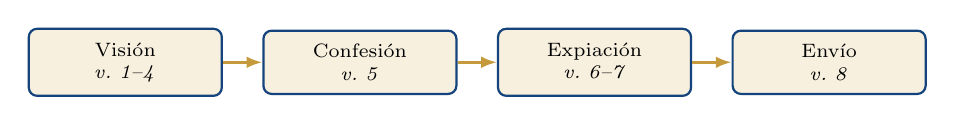
\begin{tikzpicture}[font=\scriptsize, node distance=0.5cm]
 \node[caja,text width=2.1cm,align=center] (a) {Visión\\ \emph{v.~1--4}};
 \node[caja,text width=2.1cm,align=center,right=of a] (b) {Confesión\\ \emph{v.~5}};
 \node[caja,text width=2.1cm,align=center,right=of b] (c) {Expiación\\ \emph{v.~6--7}};
 \node[caja,text width=2.1cm,align=center,right=of c] (d) {Envío\\ \emph{v.~8}};
 \foreach \i/\j in {a/b,b/c,c/d}\draw[-{Latex[length=2mm]},dorado,line width=1pt](\i)--(\j);
\end{tikzpicture}
\end{center}
\end{frame}

% ------------------------------------------------------------------
\section{Sin igual}

\begin{frame}{``No hay santo como el \SENOR''}
\begin{columns}[c,onlytextwidth]
\begin{column}{0.54\textwidth}
\begin{cita}No hay santo como \SENOR; Porque no hay ninguno fuera de ti, Y no hay refugio como el Dios nuestro.\fuente{(1~S 2:2, RVR1960)}\end{cita}
\begin{center}\heb{אֵין־קָדוֹשׁ כַּיהוָה כִּי־אֵין בִּלְתֶּךָ}\\ \heb{וְאֵין צוּר כֵּאלֹהֵינוּ}\end{center}
\small Lo canta Ana, madre de Samuel, después de recibir al hijo que pidió (1~S 1:27--2:1).
\end{column}
\begin{column}{0.44\textwidth}\scriptsize
\renewcommand{\arraystretch}{1.2}
\begin{tabular}{@{}>{\RaggedRight\arraybackslash}p{1.8cm}>{\RaggedRight\arraybackslash}p{3.6cm}@{}}
\toprule
\textbf{Término} & \textbf{Sentido} \\ \midrule
\heb{אֵין} \emph{eyn} & ``no hay'': negación de existencia. \\
\heb{כַּיהוָה} \emph{ka-Adonay} & ``como el \SENOR'': partícula de comparación \heb{כְּ}. \\
\heb{בִּלְתֶּךָ} \emph{biltéja} & ``fuera de ti'', ``excepto tú''. \\
\heb{צוּר} \emph{tsur} & ``roca''; la RVR1960 traduce ``refugio''. \\
\bottomrule
\end{tabular}\par\medskip
\small La santidad es lo que hace a Dios \destacar{incomparable}: la frase pone ``santo'' y ``no hay ninguno fuera de ti'' en paralelo.
\end{column}
\end{columns}
\end{frame}

\begin{frame}{La fórmula de lo incomparable}
\begin{columns}[t,onlytextwidth]
\begin{column}{0.49\textwidth}
\begin{cita}¿Quién como tú, oh \SENOR, entre los dioses? ¿Quién como tú, magnífico en santidad, terrible en maravillosas hazañas, hacedor de prodigios?\fuente{(Éx 15:11, RVR1960)}\end{cita}
\scriptsize\heb{מִי־כָמֹכָה בָּאֵלִם יְהוָה מִי כָּמֹכָה נֶאְדָּר בַּקֹּדֶשׁ}\par
\emph{mi jamoja} ``¿quién como tú?'': la pregunta que no tiene respuesta. \heb{נֶאְדָּר} \emph{ne'dar}: ``majestuoso, glorioso''.
\end{column}
\begin{column}{0.49\textwidth}
\begin{cita}¿A qué, pues, me haréis semejante o me compararéis? dice el Santo. Levantad en alto vuestros ojos, y mirad quién creó estas cosas; él saca y cuenta su ejército; a todas llama por sus nombres; ninguna faltará; tal es la grandeza de su fuerza, y el poder de su dominio.\fuente{(Is 40:25--26, RVR1960)}\end{cita}
\scriptsize\heb{וְאֶל־מִי תְדַמְּיוּנִי וְאֶשְׁוֶה יֹאמַר קָדוֹשׁ}\par
\heb{דמה} \emph{damah}: ``asemejar''. Aquí ``el Santo'' es el nombre de Dios. Las estrellas que el mundo antiguo adoraba son su ejército contado por nombre.
\end{column}
\end{columns}
\end{frame}

\begin{frame}{Más que el universo}
\centering
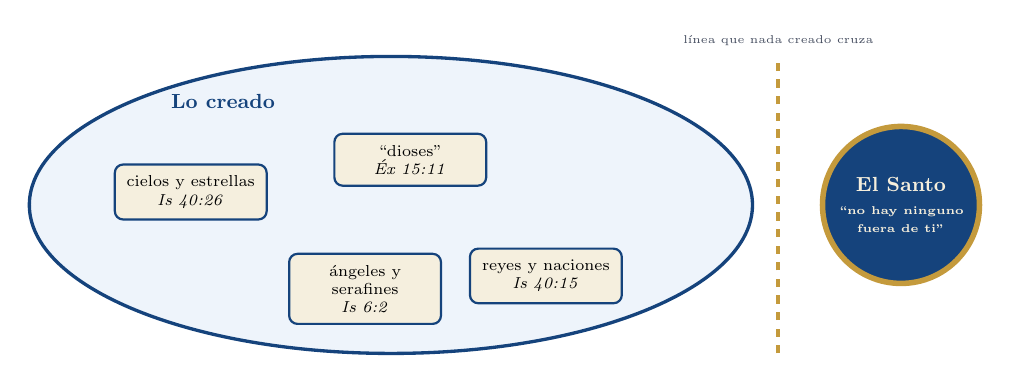
\begin{tikzpicture}[font=\scriptsize,scale=0.82,transform shape]
 \draw[azul,line width=1.2pt,fill=celeste!10] (0,0) ellipse (5.6cm and 2.3cm);
 \node[azul,font=\small\bfseries] at (-2.6,1.6) {Lo creado};
 \node[caja,text width=2.0cm,align=center] at (-3.1,0.2) {cielos y estrellas\\ \emph{Is 40:26}};
 \node[caja,text width=2.0cm,align=center] at (-0.4,-1.3) {ángeles y serafines\\ \emph{Is 6:2}};
 \node[caja,text width=2.0cm,align=center] at (2.4,-1.1) {reyes y naciones\\ \emph{Is 40:15}};
 \node[caja,text width=2.0cm,align=center] at (0.3,0.7) {``dioses''\\ \emph{Éx 15:11}};
 \node[draw=dorado,line width=2pt,fill=azul,text=papiro,circle,minimum size=2.4cm,align=center,font=\small\bfseries] (d) at (7.9,0) {El Santo\\[-1pt]{\tiny ``no hay ninguno}\\[-3pt]{\tiny fuera de ti''}};
 \draw[dorado,line width=1.4pt,dashed] (6.0,-2.3) -- (6.0,2.3);
 \node[font=\tiny,text=gris,align=center] at (6.0,2.55) {línea que nada creado cruza};
\end{tikzpicture}\par\vspace{6pt}
\begin{cita}He aquí que los cielos, los cielos de los cielos, no te pueden contener.\fuente{(1~R 8:27, RVR1960)}\end{cita}
\end{frame}

% ------------------------------------------------------------------
\section{La palabra}

\begin{frame}{La raíz \heb{קדשׁ}}
\begin{columns}[c,onlytextwidth]
\begin{column}{0.46\textwidth}
\centering
\begin{tikzpicture}[font=\scriptsize]
 \node[draw=dorado,line width=1.5pt,fill=azul,text=papiro,circle,minimum size=1.8cm,font=\large] (r) at (0,0) {\heb{קדשׁ}};
 \node[caja,text width=2.2cm,align=center] (a) at (-1.75,1.75) {\heb{קָדוֹשׁ} \emph{qadosh}\\ adj.: santo};
 \node[caja,text width=2.2cm,align=center] (b) at (1.75,1.75) {\heb{קֹדֶשׁ} \emph{qódesh}\\ sust.: santidad, lo sagrado};
 \node[caja,text width=2.2cm,align=center] (c) at (-1.75,-1.75) {\heb{קָדַשׁ} \emph{qadash}\\ verbo: ser santo; santificar, consagrar};
 \node[caja,text width=2.2cm,align=center] (d) at (1.75,-1.75) {\heb{מִקְדָּשׁ} \emph{miqdash}\\ santuario};
 \foreach \n in {a,b,c,d}\draw[dorado,line width=1pt](r)--(\n);
\end{tikzpicture}
\end{column}
\begin{column}{0.52\textwidth}\small
\begin{itemize}
\item Sentido base: lo \destacar{apartado} para Dios y distinto de lo común.
\item Su contrario es \heb{חֹל} \emph{jol}, ``profano, común'' (Lv 10:10).
\item Usos concretos: \emph{tierra santa} (Éx 3:5), \emph{lugar santísimo} (\heb{קֹדֶשׁ הַקֳּדָשִׁים}), \emph{el Santo de Israel} (\heb{קְדוֹשׁ יִשְׂרָאֵל}), título preferido de Isaías.
\end{itemize}
\precision{la etimología es discutida. Unos la relacionan con ``separar'' y otros con el acadio \emph{qadāšu}, ``ser puro, limpio'' (HALOT). El uso bíblico une ambas ideas.}
\end{column}
\end{columns}
\end{frame}

\begin{frame}{Lo santo y lo profano}
\begin{cita}para poder discernir entre lo santo y lo profano, y entre lo inmundo y lo limpio.\fuente{(Lv 10:10, RVR1960)}\end{cita}
\begin{center}\heb{וּלֲהַבְדִּיל בֵּין הַקֹּדֶשׁ וּבֵין הַחֹל וּבֵין הַטָּמֵא וּבֵין הַטָּהוֹר}\end{center}
\centering
\begin{tikzpicture}[font=\scriptsize]
 \node[caja,text width=2.2cm,align=center,fill=azul!15] (s) at (0,0) {\textbf{santo}\\ \heb{קֹדֶשׁ}};
 \node[caja,text width=2.2cm,align=center] (p) at (3.4,0) {\textbf{profano / común}\\ \heb{חֹל}};
 \node[caja,text width=2.2cm,align=center] (l) at (6.8,0) {\textbf{limpio}\\ \heb{טָהוֹר}};
 \node[caja,text width=2.2cm,align=center,fill=gris!20] (i) at (10.0,0) {\textbf{inmundo}\\ \heb{טָמֵא}};
 \draw[{Latex}-{Latex},azul,line width=1pt] (s)--node[below=3pt,font=\tiny]{separar}(p);
 \draw[{Latex}-{Latex},azul,line width=1pt] (l)--(i);
\end{tikzpicture}\par\smallskip
\small\RaggedRight El verbo \heb{הִבְדִּיל} \emph{hivdil}, ``separar'', es el mismo de Gn 1:4 (``separó Dios la luz de las tinieblas''). La santidad traza la diferencia entre Dios y todo lo demás.
\end{frame}

\begin{frame}{Del hebreo a Pablo}
\centering
\begin{tikzpicture}[font=\scriptsize,node distance=0.7cm]
 \node[caja,text width=3.1cm,align=center] (h) {\textbf{Hebreo}\\ \heb{קָדוֹשׁ} \emph{qadosh}\\ \heb{קֹדֶשׁ} \emph{qódesh}};
 \node[caja,text width=3.1cm,align=center,right=of h] (l) {\textbf{Septuaginta (LXX)}\\ \grc{ἅγιος} \emph{hágios}\\ \grc{ἁγιάζω} \emph{hagiázō}};
 \node[caja,text width=3.1cm,align=center,right=of l] (p) {\textbf{Pablo}\\ \grc{ἁγιασμός} \emph{hagiasmós}\\ \grc{ἁγιωσύνη} \emph{hagiōsýnē}};
 \draw[-{Latex[length=2.5mm]},dorado,line width=1.2pt] (h)--(l);
 \draw[-{Latex[length=2.5mm]},dorado,line width=1.2pt] (l)--(p);
 \node[below=0.35cm of l,text width=11cm,align=center,font=\scriptsize\itshape,text=gris] {La LXX traduce casi siempre \emph{qadosh} por \emph{hágios}; Pablo hereda la palabra con todo su contenido hebreo.};
\end{tikzpicture}\par\medskip
\scriptsize
\renewcommand{\arraystretch}{1.2}
\begin{tabular}{@{}>{\RaggedRight\arraybackslash}p{2.4cm}>{\RaggedRight\arraybackslash}p{9.4cm}@{}}
\toprule
\grc{ἅγιος} & ``santo''. Pablo llama ``santos'' a los creyentes (Ro 1:7; 1~Co 1:2). \\
\grc{ἁγιασμός} & ``santificación'': el proceso y el estado de ser apartado para Dios (1~Ts 4:3, 7; 1~Co 1:30) (BDAG). \\
\grc{ἁγιωσύνη} & ``santidad'' como cualidad. Solo aparece en Pablo: Ro 1:4; 2~Co 7:1; 1~Ts 3:13. \\
\bottomrule
\end{tabular}
\end{frame}

% ------------------------------------------------------------------
\section{El Nombre}

\begin{frame}{``Cuyo nombre es el Santo''}
\begin{columns}[c,onlytextwidth]
\begin{column}{0.52\textwidth}
\begin{cita}Porque así dijo el Alto y Sublime, el que habita la eternidad, y cuyo nombre es el Santo: \ldots\fuente{(Is 57:15a, RVR1960)}\end{cita}
\begin{center}\small\heb{רָם וְנִשָּׂא שֹׁכֵן עַד וְקָדוֹשׁ שְׁמוֹ}\end{center}
\end{column}
\begin{column}{0.46\textwidth}\scriptsize
\renewcommand{\arraystretch}{1.2}
\begin{tabular}{@{}>{\RaggedRight\arraybackslash}p{1.9cm}>{\RaggedRight\arraybackslash}p{3.7cm}@{}}
\toprule
\textbf{Término} & \textbf{Sentido} \\ \midrule
\heb{קָדוֹשׁ שְׁמוֹ} \emph{qadosh shemó} & ``santo (es) su nombre''. Igual en Sal 111:9 y Lc 1:49. \\
\heb{רָם וְנִשָּׂא} \emph{ram venissá} & ``alto y sublime'': los participios del trono de Is 6:1. \\
\heb{שֹׁכֵן עַד} \emph{shojen ad} & ``el que habita la eternidad''; de \heb{שׁכן} viene \emph{mishkán}, tabernáculo. \\
\heb{דַּכָּא} \emph{dakká} & ``quebrantado, molido'' (v.~15b; cf. Is 53:5). \\
\bottomrule
\end{tabular}\par\medskip
\small La santidad no se agrega al Nombre: \destacar{es el Nombre}. El que habita la eternidad habita también con el humilde.
\end{column}
\end{columns}
\end{frame}

\begin{frame}{``El Santo de Israel''}
\begin{columns}[c,onlytextwidth]
\begin{column}{0.52\textwidth}
\begin{cita}No temas, gusano de Jacob, oh vosotros los pocos de Israel; yo soy tu socorro, dice \SENOR{}; el Santo de Israel es tu Redentor.\fuente{(Is 41:14, RVR1960)}\end{cita}
\begin{center}\small\heb{וְגֹאֲלֵךְ קְדוֹשׁ יִשְׂרָאֵל}\end{center}
\scriptsize \heb{קְדוֹשׁ יִשְׂרָאֵל} \emph{qedosh Yisra'el}: el Santo ligado a un pueblo. \heb{גֹּאֲלֵךְ} \emph{go'alej}: ``tu redentor'', el pariente que rescata (Lv 25:25; Rt 4:4--6).
\begin{cita}Y guardad mis estatutos, y ponedlos por obra. Yo \SENOR{} que os santifico.\fuente{(Lv 20:8, RVR1960)}\end{cita}
\scriptsize \heb{מְקַדִּשְׁכֶם} \emph{meqaddishjem}: ``el que os santifica''. El Nombre santo hace santos.
\end{column}
\begin{column}{0.46\textwidth}
\centering
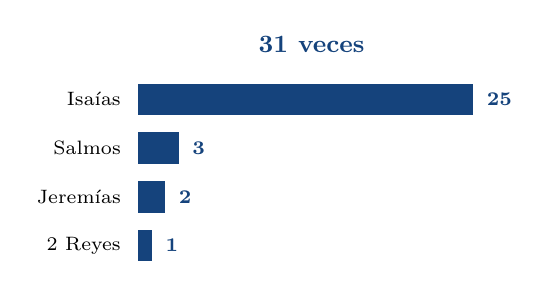
\begin{tikzpicture}[font=\scriptsize]
 \foreach \y/\l/\n in {3/Isaías/25,2/Salmos/3,1/Jeremías/2,0/2 Reyes/1}{
   \node[anchor=east] at (-0.1,\y*0.62) {\l};
   \fill[azul] (0,\y*0.62-0.2) rectangle (\n*0.17,\y*0.62+0.2);
   \node[anchor=west,font=\scriptsize\bfseries,text=azul] at (\n*0.17+0.05,\y*0.62) {\n};}
 \node[font=\small\bfseries,text=azul] at (2.2,2.55) {31 veces};
\end{tikzpicture}\par\smallskip
{\tiny\color{gris}\textit{Figura.} ``El Santo de Israel'' en el AT. \textit{Nota.} Conteo propio sobre la BHS y la RVR1960.}\par\medskip
\raggedright\scriptsize Es el título de Isaías, de 1:4 a 60:14: el profeta que vio al Santo (Is 6:3) no dejó de llamarlo así.
\end{column}
\end{columns}
\end{frame}

\begin{frame}{El Nombre santo en Cristo}
\begin{columns}[c,onlytextwidth]
\begin{column}{0.44\textwidth}
\begin{cita}Y esto erais algunos; mas ya habéis sido lavados, ya habéis sido santificados, ya habéis sido justificados en el nombre del Señor Jesús, y por el Espíritu de nuestro Dios.\fuente{(1~Co 6:11, RVR1960)}\end{cita}
\scriptsize \grc{ἡγιάσθητε}: ``fuisteis santificados'' (aoristo pasivo). Lo que Lv 20:8 atribuye al \SENOR{} que santifica, Pablo lo atribuye al \destacar{nombre del Señor Jesús}.\par\smallskip
\precision{el paralelo con Lv 20:8 es lectura propia.}
\end{column}
\begin{column}{0.54\textwidth}\scriptsize
\renewcommand{\arraystretch}{1.15}
\begin{tabular}{@{}>{\RaggedRight\arraybackslash}p{2.6cm}>{\RaggedRight\arraybackslash}p{2.0cm}>{\RaggedRight\arraybackslash}p{1.9cm}@{}}
\toprule
\textbf{Nombre} & \textbf{Original} & \textbf{Texto} \\ \midrule
Santo es su nombre & \heb{קָדוֹשׁ שְׁמוֹ} & Is 57:15 \\
El Santo de Israel & \heb{קְדוֹשׁ יִשְׂרָאֵל} & Is 41:14 \\
\SENOR{} de los ejércitos & \heb{יְהוָה צְבָאוֹת} & Is 6:3 \\
\SENOR{} que os santifico & \heb{יְהוָה מְקַדִּשְׁכֶם} & Lv 20:8 \\
El Santo de Dios & \grc{ὁ ἅγιος τοῦ θεοῦ} & Mr 1:24 \\
El Santo y el Justo & \grc{τὸν ἅγιον καὶ δίκαιον} & Hch 3:14 \\
El Santo, el Verdadero & \grc{ὁ ἅγιος, ὁ ἀληθινός} & Ap 3:7 \\
\bottomrule
\end{tabular}\par\smallskip
\precision{los sabios llaman a Dios \emph{HaQadosh Barukh Hu}, ``el Santo, bendito sea'' (p.~ej., \emph{Shemot Rabá} 3:6).}
\end{column}
\end{columns}
\end{frame}

% ------------------------------------------------------------------
\section{Definición}

\begin{frame}{¿Qué es la santidad de Dios?}
\begin{tcolorbox}[colback=papiro,colframe=azul,boxrule=1pt,arc=3pt,fonttitle=\bfseries\small,title=Definición]
\small La santidad es la perfección eterna por la cual Dios es \destacar{absolutamente distinto} de todo lo creado y \destacar{absolutamente puro} de todo mal. Es lo que lo hace único, sin igual, y lo que da a cada uno de sus atributos su carácter divino.
\end{tcolorbox}
\scriptsize\renewcommand{\arraystretch}{1.25}
\begin{tabular}{@{}>{\RaggedRight\arraybackslash}p{2.6cm}>{\RaggedRight\arraybackslash}p{5.0cm}>{\RaggedRight\arraybackslash}p{4.0cm}@{}}
\toprule
\textbf{Dimensión} & \textbf{Qué afirma} & \textbf{Textos} \\ \midrule
Majestad (trascendencia) & Dios es distinto de toda criatura; nada se le compara. & 1~S 2:2; Éx 15:11; Is 40:25 \\
Pureza (moral) & Dios es limpio de todo mal y no lo tolera. & Hab 1:13; Is 6:5 \\
Cercanía santa & El Santo habita con el humilde. & Is 57:15; Os 11:9 \\
\bottomrule
\end{tabular}\par\smallskip
\begin{center}\footnotesize
\begin{tabular}{ccc}
\textbf{Clasificación:} & Identidad (¿quién es?) & \\
\textbf{Tipo:} & incomunicable en su plenitud & comunicable como reflejo (Lv 19:2)\\
\end{tabular}
\end{center}
\end{frame}

\begin{frame}{El Alto y Sublime habita con el humilde}
\begin{cita}Porque así dijo el Alto y Sublime, el que habita la eternidad, y cuyo nombre es el Santo: Yo habito en la altura y la santidad, y con el quebrantado y humilde de espíritu, para hacer vivir el espíritu de los humildes, y para vivificar el corazón de los quebrantados.\fuente{(Is 57:15, RVR1960)}\end{cita}
\begin{cita}Muy limpio eres de ojos para ver el mal, ni puedes ver el agravio.\fuente{(Hab 1:13, RVR1960)}\end{cita}
\small ``Alto y sublime'' (\heb{רָם וְנִשָּׂא} \emph{ram venissá}) repite las palabras del trono de Is 6:1. El mismo Dios que es inalcanzable se acerca al quebrantado, tal como se acercó a Isaías con el carbón del altar.
\end{frame}

% ------------------------------------------------------------------
\section{Permea todo}

\begin{frame}{La santidad en todos sus atributos}
\centering
\begin{tikzpicture}[font=\scriptsize]
 \node[draw=dorado,line width=2pt,fill=azul,text=papiro,circle,minimum size=2.2cm,font=\normalsize\bfseries,align=center] (c) at (0,0) {SANTO\\[-2pt]{\tiny\heb{קָדוֹשׁ}}};
 \foreach \ang/\t/\r in {90/{Nombre}/{Sal 111:9},45/{Poder}/{Is 52:10},0/{Justicia}/{Is 5:16},-45/{Fidelidad}/{Sal 89:35},-90/{Celo}/{Jos 24:19},-135/{Misericordia}/{Os 11:9},180/{Sabiduría}/{Pr 9:10},135/{Eternidad}/{Is 57:15}}{
  \node[caja,text width=1.9cm,align=center] (n) at (\ang:3.0cm) {\textbf{\textcolor{azul}{\t}}\\ {\tiny\r}};
  \draw[dorado,line width=1.1pt] (c) -- (n);}
\end{tikzpicture}\par\smallskip
\small La Escritura no dice solo que Dios \emph{es} poderoso, justo o fiel: dice que su brazo es \emph{santo}, que su justicia lo muestra \emph{santo} y que jura por su \emph{santidad}.
\end{frame}

\begin{frame}{Cómo califica la santidad a cada atributo}
\scriptsize\renewcommand{\arraystretch}{1.22}
\begin{tabular}{@{}>{\RaggedRight\arraybackslash}p{1.8cm}>{\RaggedRight\arraybackslash}p{6.0cm}>{\RaggedRight\arraybackslash}p{1.5cm}>{\RaggedRight\arraybackslash}p{2.3cm}@{}}
\toprule
\textbf{Atributo} & \textbf{El texto (RVR1960)} & \textbf{Cita} & \textbf{Lo que muestra} \\ \midrule
Nombre & ``Santo y temible es su nombre.'' & Sal 111:9 & su identidad misma \\
Eternidad & ``el que habita la eternidad, y cuyo nombre es el Santo'' & Is 57:15 & eterno y santo a la vez \\
Poder & ``\SENOR{} desnudó su santo brazo ante los ojos de todas las naciones'' & Is 52:10 & poder sin abuso \\
Justicia & ``el Dios Santo será santificado con justicia'' & Is 5:16 & juicio sin corrupción \\
Fidelidad & ``Una vez he jurado por mi santidad, y no mentiré a David.'' & Sal 89:35 & jura por lo más alto que es \\
Celo & ``él es Dios santo, y Dios celoso'' & Jos 24:19 & celo sin egoísmo \\
Misericordia & ``porque Dios soy, y no hombre, el Santo en medio de ti'' & Os 11:9 & perdona \emph{porque} es santo \\
Sabiduría & ``el conocimiento del Santísimo es la inteligencia'' & Pr 9:10 & la sabiduría empieza en él \\
Verdad & ``Esto dice el Santo, el Verdadero'' & Ap 3:7 & santo y verdadero (de Cristo) \\
\bottomrule
\end{tabular}\par\smallskip
\precision{Os 11:9 es el caso más llamativo: Dios no destruye a Efraín porque es santo, ``Dios y no hombre''. Su santidad no se reduce a castigar.}
\end{frame}

\begin{frame}{Teología: la exposición de Pink}
\begin{columns}[t,onlytextwidth]
\begin{column}{0.55\textwidth}\small
Recorrido de Pink sobre la santidad (Pink, 1930/2020):
\begin{enumerate}
\item Solo Dios es santo en sí mismo; la criatura lo es por derivación (Éx 15:11; 1~S 2:2).
\item Su santidad se ve en sus obras, en su ley (Ro 7:12) y sobre todo en la cruz.
\item Porque es santo, aborrece el pecado.
\item Porque es santo, nadie es aceptado por sus propias obras.
\item Porque es santo, se le debe adorar con reverencia (Sal 89:7; 99:5).
\end{enumerate}
\end{column}
\begin{column}{0.43\textwidth}
\begin{cita}Exaltad a \SENOR{} nuestro Dios, y postraos ante su santo monte, porque \SENOR{} nuestro Dios es santo.\fuente{(Sal 99:9, RVR1960)}\end{cita}
\footnotesize El Sal 99 repite tres veces ``él es santo'' (vv.~3, 5, 9), como un trisagio en forma de estribillo.\par\smallskip
\precision{la imagen de la santidad como la ``hermosura'' de Dios que da brillo a los demás atributos viene de Charnock (1682/1996).}
\end{column}
\end{columns}
\end{frame}

% ------------------------------------------------------------------
\section{En la zarza}

\begin{frame}{Un encuentro en Israel: Moisés}
\fotolado{panel_exodo3.jpg}{Elaboración propia: Éx 3:5 en texto hebreo consonántico (BHS).}
\begin{columns}[c,onlytextwidth]
\begin{column}{0.58\textwidth}
\begin{cita}Y dijo: No te acerques; quita tu calzado de tus pies, porque el lugar en que tú estás, tierra santa es. Y dijo: Yo soy el Dios de tu padre, Dios de Abraham, Dios de Isaac, y Dios de Jacob. Entonces Moisés cubrió su rostro, porque tuvo miedo de mirar a Dios.\fuente{(Éx 3:5--6, RVR1960)}\end{cita}
\small Moisés pastorea en el desierto, junto a Horeb. Una zarza arde sin consumirse (Éx 3:1--3). Lo que hace santa la tierra no es el suelo, sino la presencia de Dios.
\end{column}
\begin{column}{0.40\textwidth}\end{column}
\end{columns}
\end{frame}

\begin{frame}{Filología de Éx 3:5}
\begin{center}\heb{שַׁל־נְעָלֶיךָ מֵעַל רַגְלֶיךָ כִּי הַמָּקוֹם אֲשֶׁר אַתָּה עוֹמֵד עָלָיו אַדְמַת־קֹדֶשׁ הוּא}\end{center}
\scriptsize\renewcommand{\arraystretch}{1.22}
\begin{tabular}{@{}>{\RaggedRight\arraybackslash}p{2.8cm}>{\RaggedRight\arraybackslash}p{1.3cm}>{\RaggedRight\arraybackslash}p{7.6cm}@{}}
\toprule
\textbf{Término} & \textbf{Raíz} & \textbf{Sentido} \\ \midrule
\heb{אַל־תִּקְרַב} \emph{al-tiqrav} & \heb{קרב} & ``no te acerques'': de la misma raíz que \emph{qorbán}, la ofrenda que ``se acerca''. A Dios solo se llega por el camino que él abre. \\
\heb{שַׁל} \emph{shal} & \heb{נשׁל} & ``quita'', ``desata''. Descalzarse era señal de respeto y de despojo ante un superior. \\
\heb{אַדְמַת־קֹדֶשׁ} \emph{admat-qódesh} & \heb{קדשׁ} & ``tierra de santidad'': construcción hebrea por adjetivo. Primera vez que aparece el sustantivo \emph{qódesh} en la Torá. \\
\bottomrule
\end{tabular}\par\medskip
\precision{el dato de la primera aparición es conteo propio: conviene verificarlo en e-Sword o en la BHS. La raíz ya aparece antes como verbo en Gn 2:3 (``lo santificó'', el sábado).}
\end{frame}

\begin{frame}{Isaías y Moisés: el mismo patrón}
\scriptsize\renewcommand{\arraystretch}{1.3}
\begin{tabular}{@{}>{\RaggedRight\arraybackslash}p{2.2cm}>{\RaggedRight\arraybackslash}p{4.8cm}>{\RaggedRight\arraybackslash}p{4.8cm}@{}}
\toprule
& \textbf{Moisés (Éx 3)} & \textbf{Isaías (Is 6)} \\ \midrule
Dios se manifiesta & fuego en la zarza (3:2) & trono, serafines ``ardientes'', humo (6:1--4) \\
Se declara santo & ``tierra santa es'' (3:5) & ``Santo, santo, santo'' (6:3) \\
El hombre se cubre & ``cubrió su rostro'' (3:6) & ``¡Ay de mí!'' (6:5); los serafines cubren su rostro (6:2) \\
Dios se acerca & ``he descendido para librarlos'' (3:8) & el carbón del altar quita la culpa (6:7) \\
Envío & ``Ven, por tanto, ahora, y te enviaré'' (3:10) & ``¿A quién enviaré?'' --- ``Envíame a mí'' (6:8) \\
\bottomrule
\end{tabular}\par\medskip
\small En los dos encuentros, la santidad primero \destacar{aparta} al hombre y luego lo \destacar{envía}. El Santo no se acerca para destruir, sino para librar.
\par\smallskip\precision{el paralelo es una lectura propia; los dos relatos comparten la secuencia de las escenas de llamado profético.}
\end{frame}

% ------------------------------------------------------------------
\section{En Cristo}

\begin{frame}{Isaías vio su gloria}
\begin{cita}Isaías dijo esto cuando vio su gloria, y habló acerca de él.\fuente{(Jn 12:41, RVR1960)}\end{cita}
\small Juan cita Is 6:10 (Jn 12:40) y afirma que la gloria que vio Isaías era la de Jesús. Es el puente entre el trono de Is 6 y Cristo.\par\medskip
\precision{el puente es de Juan, no de Pablo. Pablo llega al mismo punto por otro camino: la gloria de Dios brilla ``en la faz de Jesucristo'' (2~Co 4:6).}
\begin{cita}Porque Dios, que mandó que de las tinieblas resplandeciese la luz, es el que resplandeció en nuestros corazones, para iluminación del conocimiento de la gloria de Dios en la faz de Jesucristo.\fuente{(2~Co 4:6, RVR1960)}\end{cita}
\scriptsize\grc{δόξα} \emph{dóxa}: la palabra con que la LXX traduce \heb{כָּבוֹד}. El \emph{kavod} que llena la tierra en Is 6:3 ahora tiene un rostro.
\end{frame}

\begin{frame}{``Según el Espíritu de santidad''}
\begin{cita}que fue declarado Hijo de Dios con poder, según el Espíritu de santidad, por la resurrección de entre los muertos.\fuente{(Ro 1:4, RVR1960)}\end{cita}
\scriptsize\renewcommand{\arraystretch}{1.22}
\begin{tabular}{@{}>{\RaggedRight\arraybackslash}p{3.0cm}>{\RaggedRight\arraybackslash}p{8.8cm}@{}}
\toprule
\grc{πνεῦμα ἁγιωσύνης} & \emph{pneûma hagiōsýnēs}, ``espíritu de santidad''. Es un hebraísmo: calca \heb{רוּחַ קָדְשְׁךָ} \emph{rúaj qodshéja}, ``tu santo espíritu'' (Sal 51:11 [51:13]; Is 63:10--11). \\
\grc{ἁγιωσύνη} & sustantivo de cualidad, propio de Pablo. Aquí, el ámbito santo de Dios en el que Cristo es declarado Hijo. \\
\bottomrule
\end{tabular}\par\medskip
\small Pablo, judío formado en las Escrituras, usa una expresión hebrea para presentar a Jesús: el Mesías resucitado pertenece a la esfera de lo santo.\par\smallskip
\precision{se discute si ``Espíritu de santidad'' es el Espíritu Santo o el espíritu de Cristo (Moo, 1996; Dunn, 1998).}
\end{frame}

\begin{frame}{El carbón del altar y la cruz}
\centering
\begin{tikzpicture}[font=\scriptsize,node distance=0.45cm]
 \node[caja,text width=2.4cm,align=center] (i1) {inmundo de labios\\ \emph{Is 6:5}};
 \node[caja,text width=2.4cm,align=center,right=of i1] (i2) {carbón del altar\\ \emph{Is 6:6}};
 \node[caja,text width=2.4cm,align=center,right=of i2] (i3) {\heb{תְּכֻפָּר} ``es expiado''\\ \emph{Is 6:7}};
 \node[caja,text width=2.4cm,align=center,right=of i3] (i4) {``envíame a mí''\\ \emph{Is 6:8}};
 \node[caja,text width=2.4cm,align=center,below=1.0cm of i1,fill=azul!12] (p1) {``destituidos de la gloria''\\ \emph{Ro 3:23}};
 \node[caja,text width=2.4cm,align=center,right=of p1,fill=azul!12] (p2) {Cristo, \grc{ἱλαστήριον}\\ \emph{Ro 3:25}};
 \node[caja,text width=2.4cm,align=center,right=of p2,fill=azul!12] (p3) {santificados, justificados\\ \emph{1~Co 6:11}};
 \node[caja,text width=2.4cm,align=center,right=of p3,fill=azul!12] (p4) {embajadores\\ \emph{2~Co 5:20}};
 \foreach \a/\b in {i1/i2,i2/i3,i3/i4,p1/p2,p2/p3,p3/p4}\draw[-{Latex[length=2mm]},dorado,line width=1pt](\a)--(\b);
 \foreach \n in {1,2,3,4}\draw[densely dotted,azul,line width=0.8pt](i\n)--(p\n);
 \node[left=0.15cm of i1,rotate=90,anchor=south,font=\tiny\bfseries,text=azul] {Isaías};
 \node[left=0.15cm of p1,rotate=90,anchor=south,font=\tiny\bfseries,text=azul] {Pablo};
\end{tikzpicture}\par\medskip
\begin{cita}a quien Dios puso como propiciación por medio de la fe en su sangre, para manifestar su justicia\ldots{} a fin de que él sea el justo, y el que justifica al que es de la fe de Jesús.\fuente{(Ro 3:25--26, RVR1960)}\end{cita}
\scriptsize Cadena léxica: \heb{כפר} (Is 6:7) $\rightarrow$ \heb{כַּפֹּרֶת} \emph{kapporet} $\rightarrow$ LXX \grc{ἱλαστήριον} (Éx 25:17) $\rightarrow$ Ro 3:25.\quad
\precision{la correspondencia es tipológica; Pablo no cita Is 6 en Romanos 3.}
\end{frame}

\begin{frame}{Cristo, nuestra santificación}
\begin{columns}[t,onlytextwidth]
\begin{column}{0.49\textwidth}
\begin{cita}Mas por él estáis vosotros en Cristo Jesús, el cual nos ha sido hecho por Dios sabiduría, justificación, santificación y redención.\fuente{(1~Co 1:30, RVR1960)}\end{cita}
\begin{cita}Y esto erais algunos; mas ya habéis sido lavados, ya habéis sido santificados, ya habéis sido justificados en el nombre del Señor Jesús, y por el Espíritu de nuestro Dios.\fuente{(1~Co 6:11, RVR1960)}\end{cita}
\end{column}
\begin{column}{0.49\textwidth}
\begin{cita}en su cuerpo de carne, por medio de la muerte, para presentaros santos y sin mancha e irreprensibles delante de él.\fuente{(Col 1:22, RVR1960)}\end{cita}
\scriptsize\grc{ἁγιασμός} (1~Co 1:30): la santidad no es primero un logro, es Cristo dado. El versículo siguiente cita Jer 9:24: ``El que se gloría, gloríese en el Señor'' (1~Co 1:31), el verso que une esta obra.\par\smallskip
\precision{la autoría paulina de Colosenses es discutida; la misma idea está en cartas indiscutidas (1~Co 6:11; 1~Ts 3:13).}
\end{column}
\end{columns}
\end{frame}

\begin{frame}{La plenitud santa habita en Cristo}
\begin{cita}Porque en él habita corporalmente toda la plenitud de la Deidad.\fuente{(Col 2:9, RVR1960)}\end{cita}
\centering
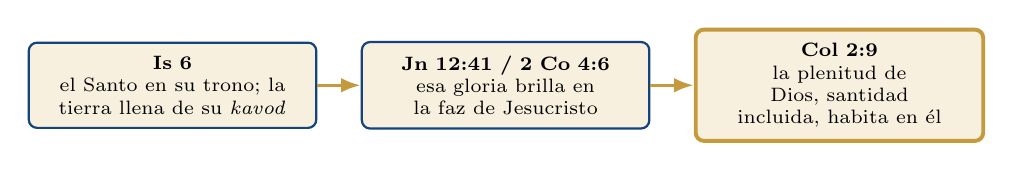
\begin{tikzpicture}[font=\scriptsize,node distance=0.55cm]
 \node[caja,text width=3.3cm,align=center] (a) {\textbf{Is 6}\\ el Santo en su trono; la tierra llena de su \emph{kavod}};
 \node[caja,text width=3.3cm,align=center,right=of a] (b) {\textbf{Jn 12:41 / 2~Co 4:6}\\ esa gloria brilla en la faz de Jesucristo};
 \node[caja,text width=3.3cm,align=center,right=of b,draw=dorado,line width=1.4pt] (c) {\textbf{Col 2:9}\\ la plenitud de Dios, santidad incluida, habita en él};
 \draw[-{Latex[length=2.5mm]},dorado,line width=1.2pt](a)--(b);
 \draw[-{Latex[length=2.5mm]},dorado,line width=1.2pt](b)--(c);
\end{tikzpicture}\par\medskip
\small\RaggedRight Cristo es ``el Santo y el Justo'' (Hch 3:14). En él, el Dios que Isaías no podía mirar sin morir se deja ver, y el carbón que quema se convierte en perdón.
\end{frame}

% ------------------------------------------------------------------
\section{Vivirlo}

\begin{frame}{Santos, porque él es santo}
\begin{columns}[t,onlytextwidth]
\begin{column}{0.49\textwidth}
\begin{cita}Santos seréis, porque santo soy yo \SENOR{} vuestro Dios.\fuente{(Lv 19:2, RVR1960)}\end{cita}
\begin{center}\small\heb{קְדֹשִׁים תִּהְיוּ כִּי קָדוֹשׁ אֲנִי}\\ \heb{יְהוָה אֱלֹהֵיכֶם}\end{center}
\end{column}
\begin{column}{0.49\textwidth}
\begin{cita}sino, como aquel que os llamó es santo, sed también vosotros santos en toda vuestra manera de vivir; porque escrito está: Sed santos, porque yo soy santo.\fuente{(1~P 1:15--16, RVR1960)}\end{cita}
\end{column}
\end{columns}
\small El mandato tiene un fundamento: \heb{כִּי} \emph{ki}, ``porque''. Somos santos \emph{porque} él lo es. La santidad humana es reflejo, no origen.\par\smallskip
\begin{cita}Pues no nos ha llamado Dios a inmundicia, sino a santificación.\fuente{(1~Ts 4:7, RVR1960)}\end{cita}
\end{frame}

\begin{frame}{Cinco respuestas a la santidad}
\centering
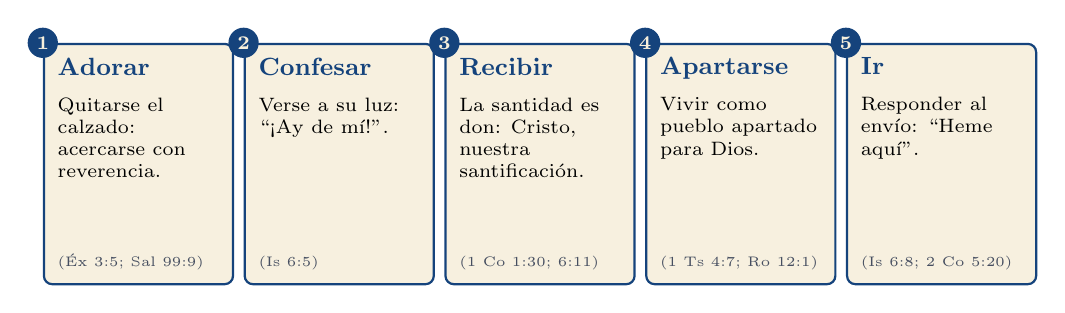
\begin{tikzpicture}
 \foreach \x/\n/\t/\d/\r in {0/1/{Adorar}/{Quitarse el calzado: acercarse con reverencia.}/{Éx 3:5; Sal 99:9},
   2.55/2/{Confesar}/{Verse a su luz: ``¡Ay de mí!''.}/{Is 6:5},
   5.1/3/{Recibir}/{La santidad es don: Cristo, nuestra santificación.}/{1 Co 1:30; 6:11},
   7.65/4/{Apartarse}/{Vivir como pueblo apartado para Dios.}/{1 Ts 4:7; Ro 12:1},
   10.2/5/{Ir}/{Responder al envío: ``Heme aquí''.}/{Is 6:8; 2 Co 5:20}}{
  \node[caja,anchor=north] (b\n) at (\x,0) {\parbox[t][2.7cm][t]{2.05cm}{\RaggedRight
    {\small\textbf{\textcolor{azul}{\t}}}\\[5pt]\scriptsize \d\par\vfill{\tiny\color{gris}(\r)}}};
  \node[circle,fill=azul,text=papiro,font=\scriptsize\bfseries,inner sep=1.6pt] at (b\n.north west) {\n};}
\end{tikzpicture}\par\medskip
\small\RaggedRight ¿Qué ``tierra santa'' pisas hoy sin darte cuenta? ¿Cuándo fue la última vez que la santidad de Dios te hizo callar antes de hablar?
\end{frame}

% ------------------------------------------------------------------
\section{Síntesis}

\begin{frame}{Síntesis}
\begin{tcolorbox}[colback=papiro,colframe=azul,boxrule=1pt,arc=3pt]
\small Dios es \destacar{santo}: absolutamente distinto de todo lo creado y puro de todo mal. ``No hay santo como el \SENOR'' (1~S 2:2). Su santidad lo hace sin igual y da a cada atributo su sello: su brazo es santo, su justicia lo muestra santo, jura por su santidad y perdona porque es ``Dios y no hombre''. El trono que vio Isaías es el de Cristo (Jn 12:41), en cuya faz brilla la gloria de Dios (2~Co 4:6), y en quien habita toda la plenitud (Col 2:9).
\end{tcolorbox}
\scriptsize\renewcommand{\arraystretch}{1.2}
\begin{tabular}{@{}>{\RaggedRight\arraybackslash}p{2.4cm}>{\RaggedRight\arraybackslash}p{9.4cm}@{}}
\toprule
\textbf{Mirada} & \textbf{Aporte} \\ \midrule
Hebrea & \emph{qadosh}: lo apartado; el trisagio; ``¿quién como tú?''; la tierra santa de la zarza. \\
Pink & solo Dios es santo en sí mismo; aborrece el pecado; exige reverencia; se ve en la cruz. \\
Paulina & \emph{hagiōsýnē} en Cristo resucitado; la gloria en su rostro; la expiación; Cristo, nuestra santificación. \\
\bottomrule
\end{tabular}
\end{frame}

\begin{frame}{Para la reflexión}
\begin{cita}Mas alábese en esto el que se hubiere de alabar: en entenderme y conocerme, que yo soy \SENOR, que hago misericordia, juicio y justicia en la tierra; porque estas cosas quiero, dice \SENOR.\fuente{(Jer 9:24, RVR1960)}\end{cita}
\small
\begin{itemize}
\item ¿Mi imagen de Dios tiene el peso (\emph{kavod}) del trono de Isaías, o es un Dios a mi medida?
\item ¿Qué ``labios inmundos'' necesita tocar hoy el carbón del altar?
\item ¿Vivo mi santificación como esfuerzo propio o como don recibido en Cristo (1~Co 1:30)?
\item Si el Santo dice ``¿a quién enviaré?'', ¿qué responde mi vida?
\end{itemize}
\end{frame}

% ------------------------------------------------------------------
\section{Glosario}

\begin{frame}{Glosario}
\scriptsize
\begin{columns}[t,onlytextwidth]
\begin{column}{0.49\textwidth}
\begin{description}\setlength{\itemsep}{1pt}
\item[\emph{Adonay}] (\heb{אֲדֹנָי}) ``Señor''; lectura judía del tetragrama.
\item[\emph{Hagiasmós}] (\grc{ἁγιασμός}) santificación: ser apartado para Dios.
\item[\emph{Hagiōsýnē}] (\grc{ἁγιωσύνη}) santidad como cualidad; solo en Pablo.
\item[\emph{Hilastērion}] (\grc{ἱλαστήριον}) propiciatorio; propiciación (Ro 3:25).
\item[\emph{Jol}] (\heb{חֹל}) lo profano o común; contrario de lo santo.
\item[\emph{Kapporet}] (\heb{כַּפֹּרֶת}) tapa del arca, el propiciatorio.
\item[\emph{Kavod}] (\heb{כָּבוֹד}) gloria; de la raíz ``ser pesado''.
\end{description}
\end{column}
\begin{column}{0.49\textwidth}
\begin{description}\setlength{\itemsep}{1pt}
\item[\emph{Kipper}] (\heb{כִּפֶּר}) expiar, cubrir la culpa.
\item[\emph{Qadosh}] (\heb{קָדוֹשׁ}) santo, apartado.
\item[\emph{Qódesh}] (\heb{קֹדֶשׁ}) santidad; lo sagrado.
\item[\emph{Serafim}] (\heb{שְׂרָפִים}) ``los ardientes'' (Is 6:2).
\item[\emph{Tetragrama}] (\heb{יהוה}) el nombre propio de Dios; aquí, \SENOR.
\item[Trisagio] la triple aclamación ``Santo, santo, santo'' (Is 6:3; Ap 4:8).
\item[\emph{Tseva'ot}] (\heb{צְבָאוֹת}) ``ejércitos''.
\item[\emph{Tsur}] (\heb{צוּר}) roca (1~S 2:2).
\end{description}
\end{column}
\end{columns}
\end{frame}

% ------------------------------------------------------------------
\section{Referencias}

\begin{frame}{Referencias}
\fontsize{6.3}{7.4}\selectfont
\refapa{Bauer, W., Danker, F.~W., Arndt, W.~F., \& Gingrich, F.~W. (2000). \emph{A Greek-English lexicon of the New Testament and other early Christian literature} (3.ª ed.). University of Chicago Press. [BDAG]}
\refapa{\emph{Biblia Reina-Valera 1960}. (1960). Sociedades Bíblicas en América Latina.}
\refapa{Charnock, S. (1996). \emph{The existence and attributes of God} (Vols. 1--2). Baker Books. (Obra original publicada en 1682)}
\refapa{Dunn, J.~D.~G. (1998). \emph{The theology of Paul the apostle}. Eerdmans.}
\refapa{Elliger, K., \& Rudolph, W. (Eds.). (1997). \emph{Biblia Hebraica Stuttgartensia} (5.ª ed.). Deutsche Bibelgesellschaft.}
\refapa{Koehler, L., \& Baumgartner, W. (2001). \emph{The Hebrew and Aramaic lexicon of the Old Testament} (M.~E.~J. Richardson, Trad.; Ed. de estudio). Brill. [HALOT]}
\refapa{Moo, D.~J. (1996). \emph{The epistle to the Romans}. Eerdmans.}
\refapa{Nestle, E., \& Aland, K. (2012). \emph{Novum Testamentum Graece} (28.ª ed.). Deutsche Bibelgesellschaft.}
\refapa{Oswalt, J.~N. (1986). \emph{The book of Isaiah: Chapters 1--39}. Eerdmans.}
\refapa{Otto, R. (1980). \emph{Lo santo: Lo racional y lo irracional en la idea de Dios} (F. Vela, Trad.). Alianza Editorial. (Obra original publicada en 1917)}
\refapa{Pink, A.~W. (2020). \emph{Los atributos de Dios}. Chapel Library. (Obra original publicada en 1930)}
\refapa{Rahlfs, A., \& Hanhart, R. (Eds.). (2006). \emph{Septuaginta} (Ed. rev.). Deutsche Bibelgesellschaft.}
\par\medskip{\color{gris}Las citas bíblicas son de la Reina-Valera 1960; ``Jehová'' se reemplaza por \SENOR. El texto hebreo es de la BHS y el griego, de NA28 y la LXX de Rahlfs-Hanhart.}
\end{frame}

\end{document}
